\documentclass{beamer}

\mode<presentation>
{
  \usetheme{Madrid}      % or try Darmstadt, Madrid, Warsaw, ...
  \usecolortheme{beaver} % or try albatross, beaver, crane, ...
  \usefonttheme{default}  % or try serif, structurebold, ...
  \setbeamertemplate{navigation symbols}{}
  \setbeamertemplate{caption}[numbered]
}

\hypersetup{
  colorlinks = true,
  urlcolor=blue,
}

\usepackage[english]{babel}
\usepackage{lmodern}% http://ctan.org/pkg/lm
\usepackage{transparent}

% Tikz stuff.
\usepackage{tikz}
\usepackage{tikz-cd}
\usepackage{pgfplots}
\usepackage{graphicx,latexsym}
\graphicspath{{./pics}}
\pgfplotsset{compat=1.16}
%\tikzstyle{ball} = [circle,shading=ball, ball color=black,
%    minimum size=1mm,inner sep=1.3pt]
%\usetikzlibrary{arrows.meta}
%\tikzset{>={Latex[length=2mm,width=1.5mm]}}
\usepgfplotslibrary{fillbetween}
\usetikzlibrary{decorations.pathreplacing}
\tikzset{
  labr/.style={anchor=north, rotate=90, inner sep=.7mm}
}
\tikzset{
  labl/.style={anchor=south, rotate=90, inner sep=.7mm}
}
\usetikzlibrary{positioning}
%\usetikzlibrary{graphs,graphs.standard}
\usetikzlibrary{decorations.pathmorphing}
\usetikzlibrary{decorations.pathreplacing}
\usetikzlibrary{arrows.meta,calc}
\usetikzlibrary{bending}
\usetikzlibrary{decorations.markings,shapes.geometric}
\tikzset{->-/.style={decoration={markings, mark=at position #1 with
{\arrow{>}}},postaction={decorate}}}
\tikzset{-|-/.style={decoration={markings, mark=at position #1 with
{\arrow{stealth}}},postaction={decorate}}}
\tikzset{movearrow/.style 2 args ={
    decoration={markings,
      mark= at position {#1} with {\arrow{#2}} ,
    },
    postaction={decorate}
  }
}
\tikzset{<--/.style={decoration={markings, mark=at position #1 with
{\arrow{<}}},postaction={decorate}}}
\tikzstyle{ball} = [circle,shading=ball, ball color=black,
minimum size=1mm,inner sep=1.3pt]
\tikzstyle{bball} = [circle,shading=ball, ball color=blue,
minimum size=1mm,inner sep=1.3pt]
\tikzstyle{miniball} = [circle,shading=ball, ball color=black,
minimum size=1mm,inner sep=0.5pt]
\tikzstyle{redminiball} = [circle,shading=ball, ball color=red,
minimum size=1mm,inner sep=0.5pt]
\tikzstyle{mminiball} = [circle,shading=ball, ball color=black,
minimum size=0.6mm,inner sep=0.1pt]
\tikzstyle{mycircle} = [draw,circle, minimum size=1mm,inner sep=1.3pt]

\newcommand{\N}{\mathbb{N}}
\newcommand{\Z}{\mathbb{Z}}
\newcommand{\Q}{\mathbb{Q}}
\newcommand{\R}{\mathbb{R}}
\newcommand{\C}{\mathbb{C}}
\newcommand{\E}{\mathbb{E}}

\DeclareMathOperator{\Span}{\mathrm{Span}}
\DeclareMathOperator{\rk}{\mathrm{rank}}
\DeclareMathOperator{\id}{\mathrm{id}}
\DeclareMathOperator{\tr}{tr}
\DeclareMathOperator{\rspace}{\mathrm{rowspace}}
\DeclareMathOperator{\rrk}{\mathrm{rowrank}}
\DeclareMathOperator{\cspace}{\mathrm{colspace}}
\DeclareMathOperator{\crk}{\mathrm{colrank}}
\DeclareMathOperator{\im}{im}
\DeclareMathOperator{\cok}{cok}
\DeclareMathOperator{\diag}{diag}
\DeclareMathOperator{\GL}{GL}
\DeclareMathOperator{\sgn}{\mathrm{sgn}}
\DeclareMathOperator{\outdeg}{\mathrm{outdeg}}
\DeclareMathOperator{\supp}{\mathrm{supp}}
\DeclareMathOperator{\vol}{\mathrm{vol}}

\definecolor{myblue}{rgb}{0.2,0.2,0.7}
\definecolor{psucolor}{rgb}{0.43,0.55,0.14}
\definecolor{reedcolor}{RGB}{169,14,19}
\setbeamercolor{frametitle}{fg=reedcolor,bg=white}
\setbeamertemplate{itemize item}{\color{reedcolor}$\blacktriangleright$}
\setbeamertemplate{itemize subitem}{\color{reedcolor}$\blacktriangleright$}

\newcommand{\bigspace}{\vspace{10pt}\pause}

\title[Deep Learning Final Project]{\bf\huge
\textcolor{reedcolor}{Deep Learning Final Project}}
\date{\textcolor{reedcolor}{May 12, 2025}}
%\titlegraphic{{\includegraphics[height=1.8in]{hyperplane_arrangement.png}}}
\makeatletter
\setbeamertemplate{title
page}[default][left,colsep=-4bp,rounded=true,shadow=\beamer@themerounded@shadow]
\makeatother

\begin{document}

\begin{frame}
  \maketitle
\end{frame}

\begin{frame}{Predicting Temperature Anomalies}

  My project was to predict future temperature anomalies---i.e. the global
  temperature difference from the average for a day.\pause In essence, this is
  a time series modelling problem where we have $1$-dimensional data and we
  want to predict what comes next in the series.

  \begin{center}
    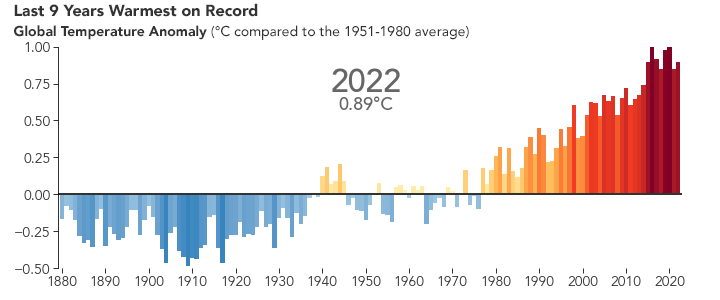
\includegraphics[scale=0.4]{global_gis_2022_chart.png}
  \end{center}

\end{frame}

\begin{frame}{How to Do This}

  In order to do this, I needed a dataset. UC Berkeley has temperature anomaly
  information ranging from $1880$ to $2022$. This was used to make the graphic
  you saw on the last slide.

  \bigspace

  From there, we need a model. Because this is a time series problem, we want a
  network which cares about the order of our elements. \pause I started with an
  LSTM model which became too cumbersome. File sizes were too large and there
  was a tendency to overfit.

  \bigspace

  I settled on a temporal convolutional network. These took less time to train,
  had smaller file sizes and were less prone to overfitting.

\end{frame}

\begin{frame}{Results}

  The results were pretty good! Overfitting was much lower on a
  reasonably-sized network, network sizes were kept down and they were
  relatively quick to train.\pause Here, the red line is the prediction and the
  blue line is our actual data set.

  \begin{center}
    \begin{figure}
      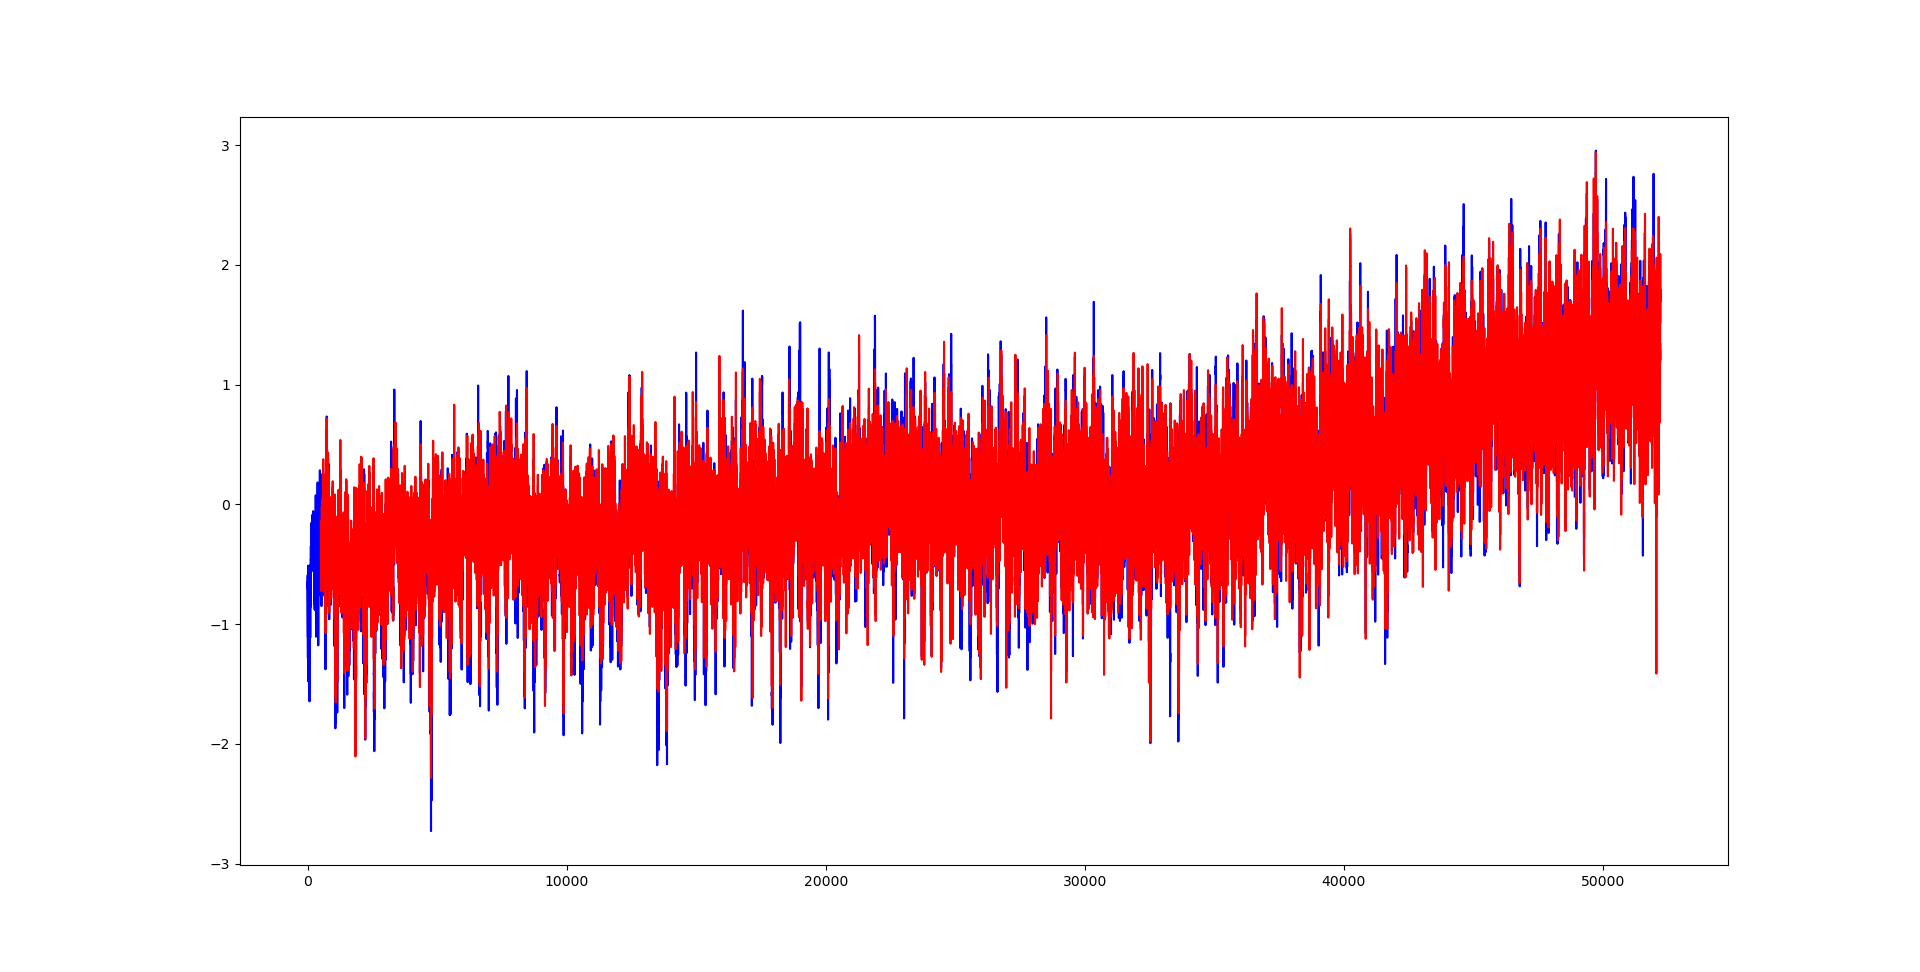
\includegraphics[scale=0.17]{accurate_predictions.png}
      \caption{Predictions v. actual data}
    \end{figure}
  \end{center}

\end{frame}

\begin{frame}{Results (cont.)}

  Unfortunately, my networks were quite horrific at actually forecasting.\pause

  \begin{center}
    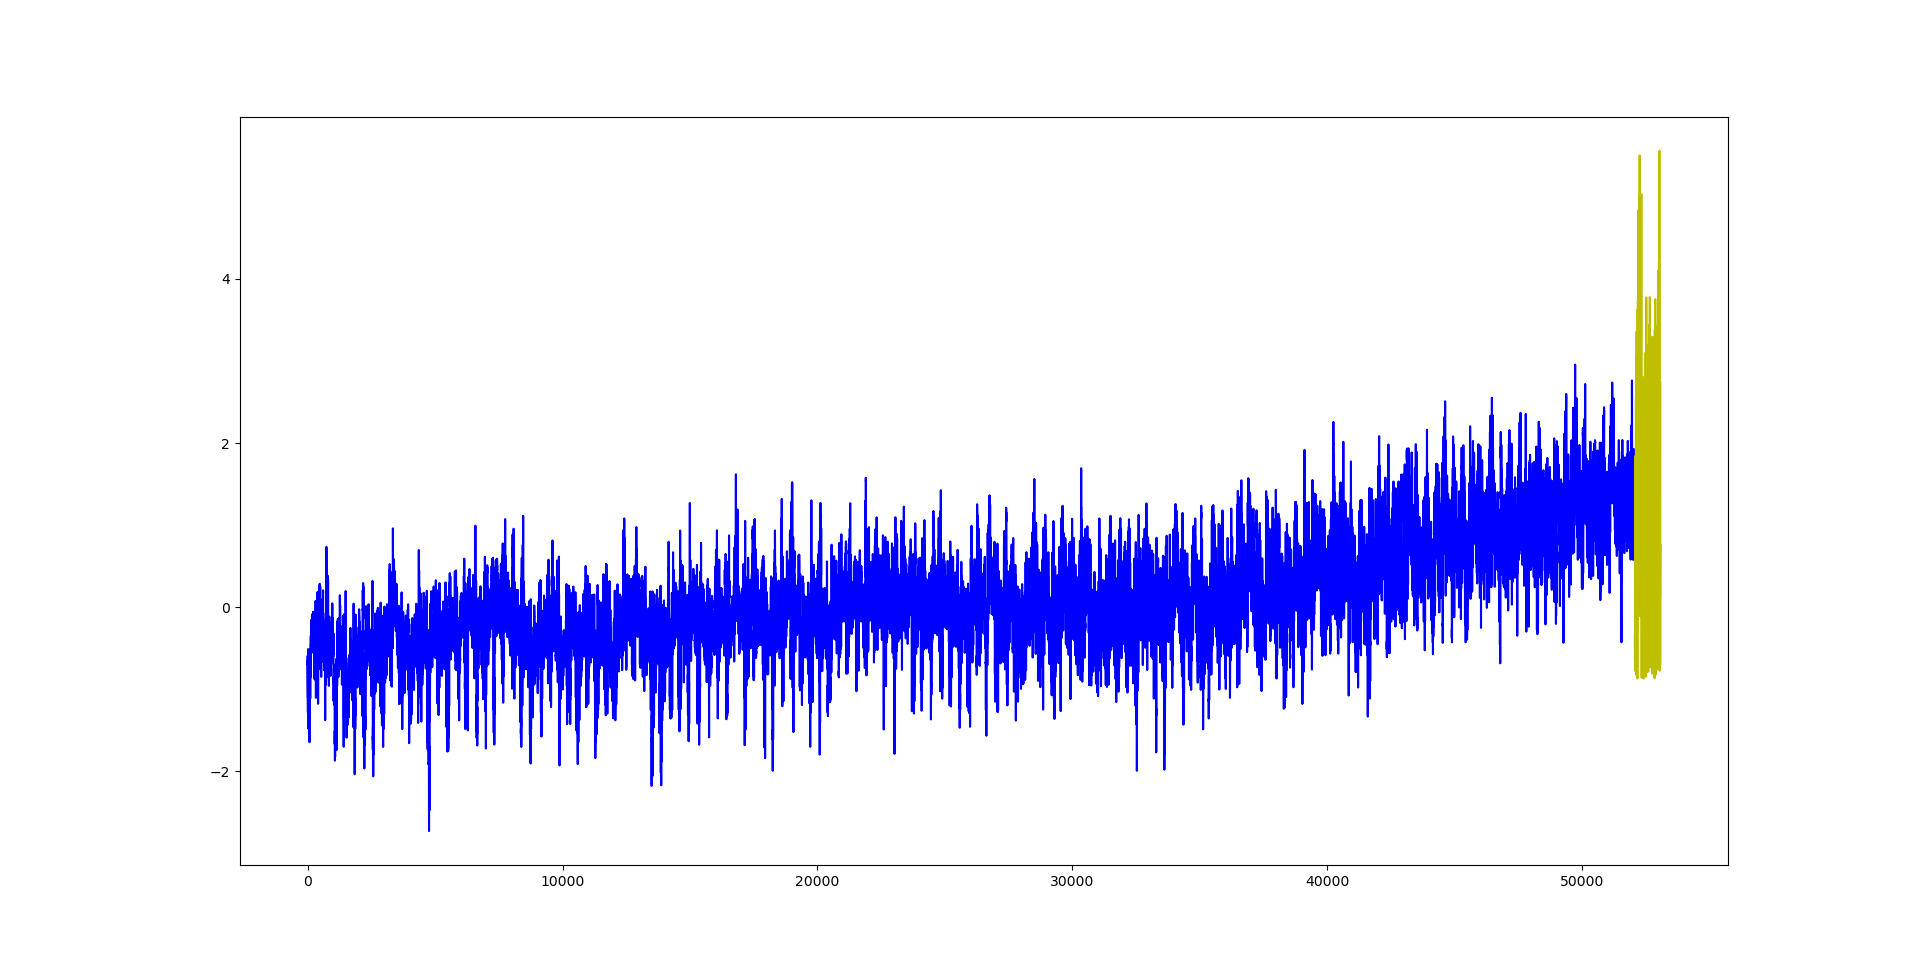
\includegraphics[scale=0.14]{erratic_predictions.png}
  \end{center}

  \begin{center}
    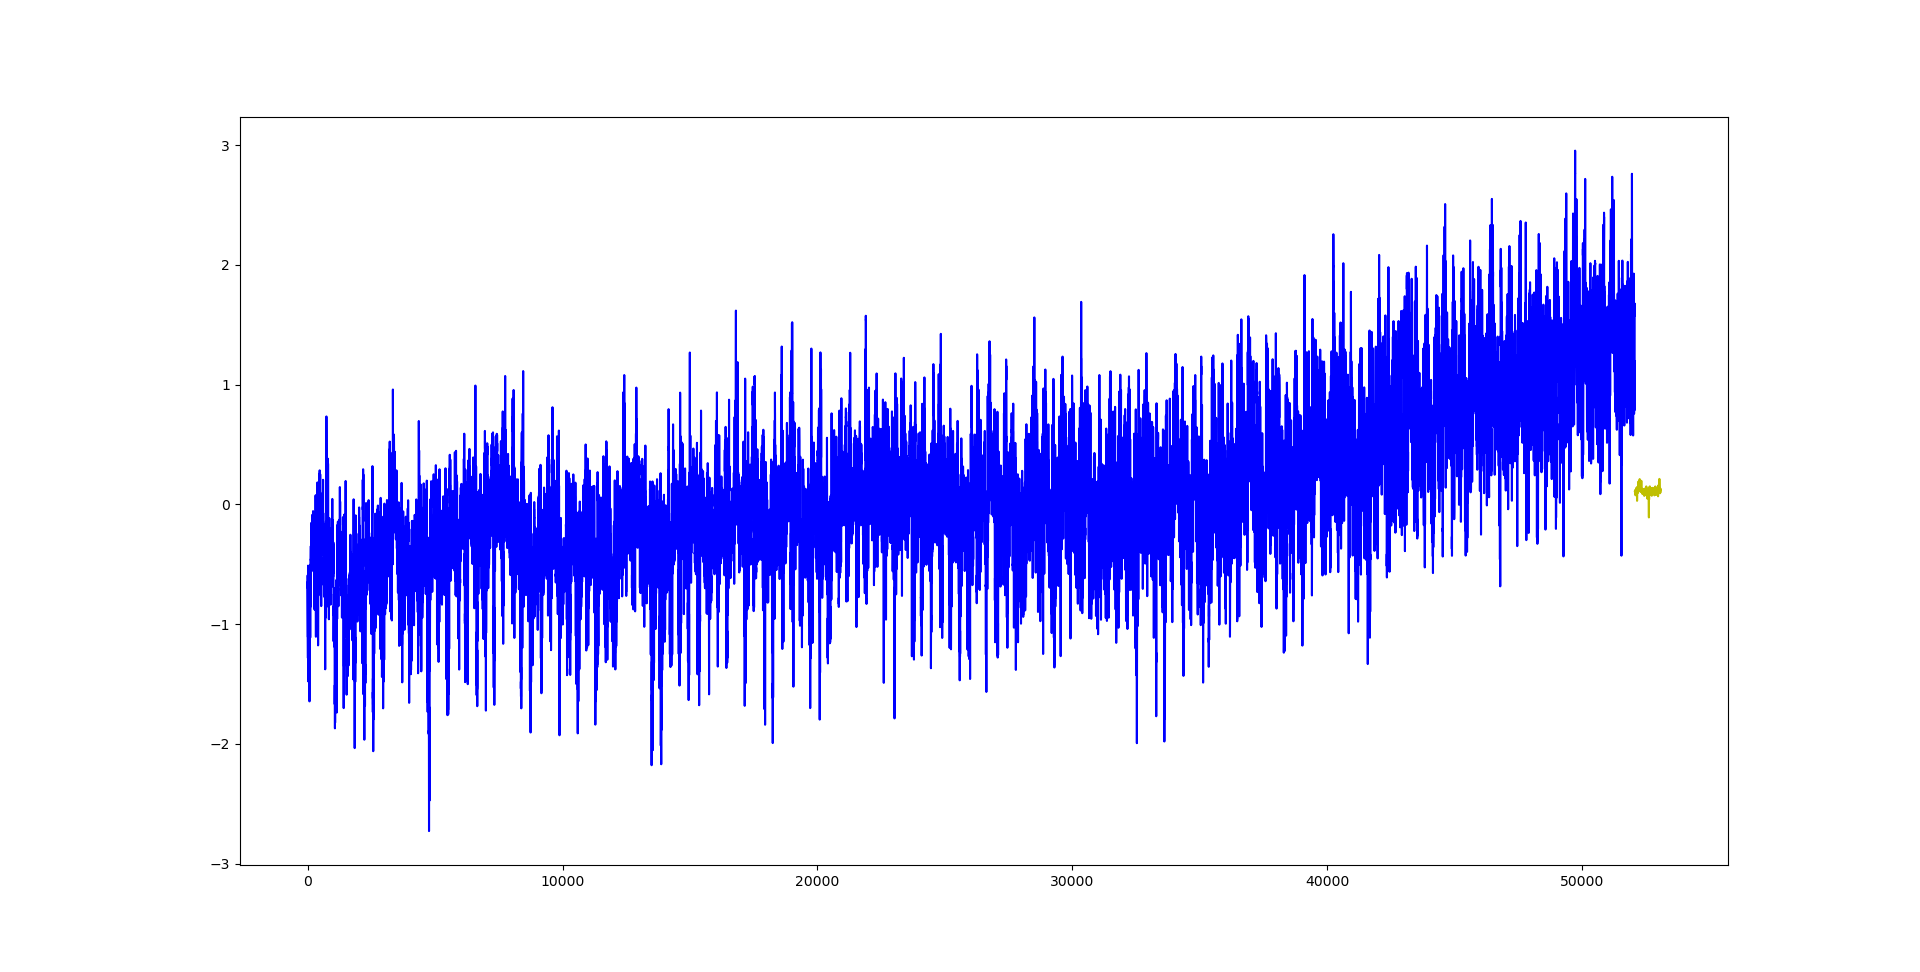
\includegraphics[scale=0.14]{squash_predictions.png}
  \end{center}

\end{frame}

\end{document}
